\chapter{Descrizione del Progetto}
un piccolo robot rover dotato di due ruote, con in quale è possibile interagire via internet attraverso una chat telegram,  inoltre ha un sensore di distanza che può individuare se ci sono ostacoli davanti  ed è dotatato di una videocamera con la quale può vedere e comunicare via chat cosa sta vedendo. oltre inviare le foto.
% **************************** Define Graphics Path **************************
\ifpdf
    \graphicspath{{Chapter3/Figs/Raster/}{Chapter3/Figs/PDF/}{Chapter3/Figs/}}
\else
    \graphicspath{{Chapter3/Figs/Vector/}{Chapter3/Figs/}}
\fi
\section{Implementazione Hardware}
Dopo aver collegato la Camera al Raspberry come mostrato nella figura

Connetto RaspberryPi alla breadboard con utilizzato un cavo flat 40 fili ed un T-Cobbler. 
in modo   porte GPIO siano accessibili direttamente nella breadboard. Sfrutto i lati esterni della breadboard per poter sfruttare una linea di alimentazione 5v ed un'altra a 3.3v

Quindi unisco i Pin 02 e il Pin06 alle linee esterne su lato della breadboard in modo da avere una linea a 5v e collego i pin 01 e 09 l’altro lato esterno per avere un’altra linea 3.3v
Così come mostrato nel disegno

Per collegare i motori delle ruote al sistema utilizzo il componente L298N come driver dei motori, l L298N è stato progettato per supportare un’unica fonte di alimentazione o per entrambi i motori e il microcontrollore. Per alimentare questo controller e i motori ho utilizzato 4 batterie AA in modo da non caricare troppo l’alimentazione del raspberry.
Collego  4 pin GPIO del Rpi ai pin di ingresso 4 motore sul L298N. 
•	IN1 e IN2 controllano la direzione del motore A e IN3 e IN4 controllano la direzione del motore B. 
o	IN1 -> GPIO 27/13 fisico
o	IN2 -> GPIO 22/15 fisico
o	IN3 -> GPIO 5 / fisica 29
o	IN4 -> GPIO 6/31 fisico
le connessioni dovrebbero corrispondere a questo schema:

L'HC-SR04 come descritto precendentemnte dispone di 4 pin - VCC, Trig, Echo, e GND.

Collego VCC alla linea di distribuzione 5v sulla breadboard, collego il pin trig al Raspberry GPIO23/Pin Fisico 16. Collego il pin Echo, tra il GPIO24/pin fisico 18 metto una resistenanza 1k OHM, infine collego un’altra resistenza tra il Pin GND alla linea Ground della breastboard e collego la linea echo con la linea del sensore 2,2K ohtm, questo perché RPI vuole 3.3v su pin GPIO  mentre il sensore fornisce una tensione 5v.
Al termine del collegament di questo sensore lo schema sarà:

Utilizzo un PowerBank a 6000ma per l’alimentazione del raspberry, ed uso come Chassis il supporto mostrato dalla figura
\begin{landscape}
	\begin{figure}[htbp!] 
		\centering    
		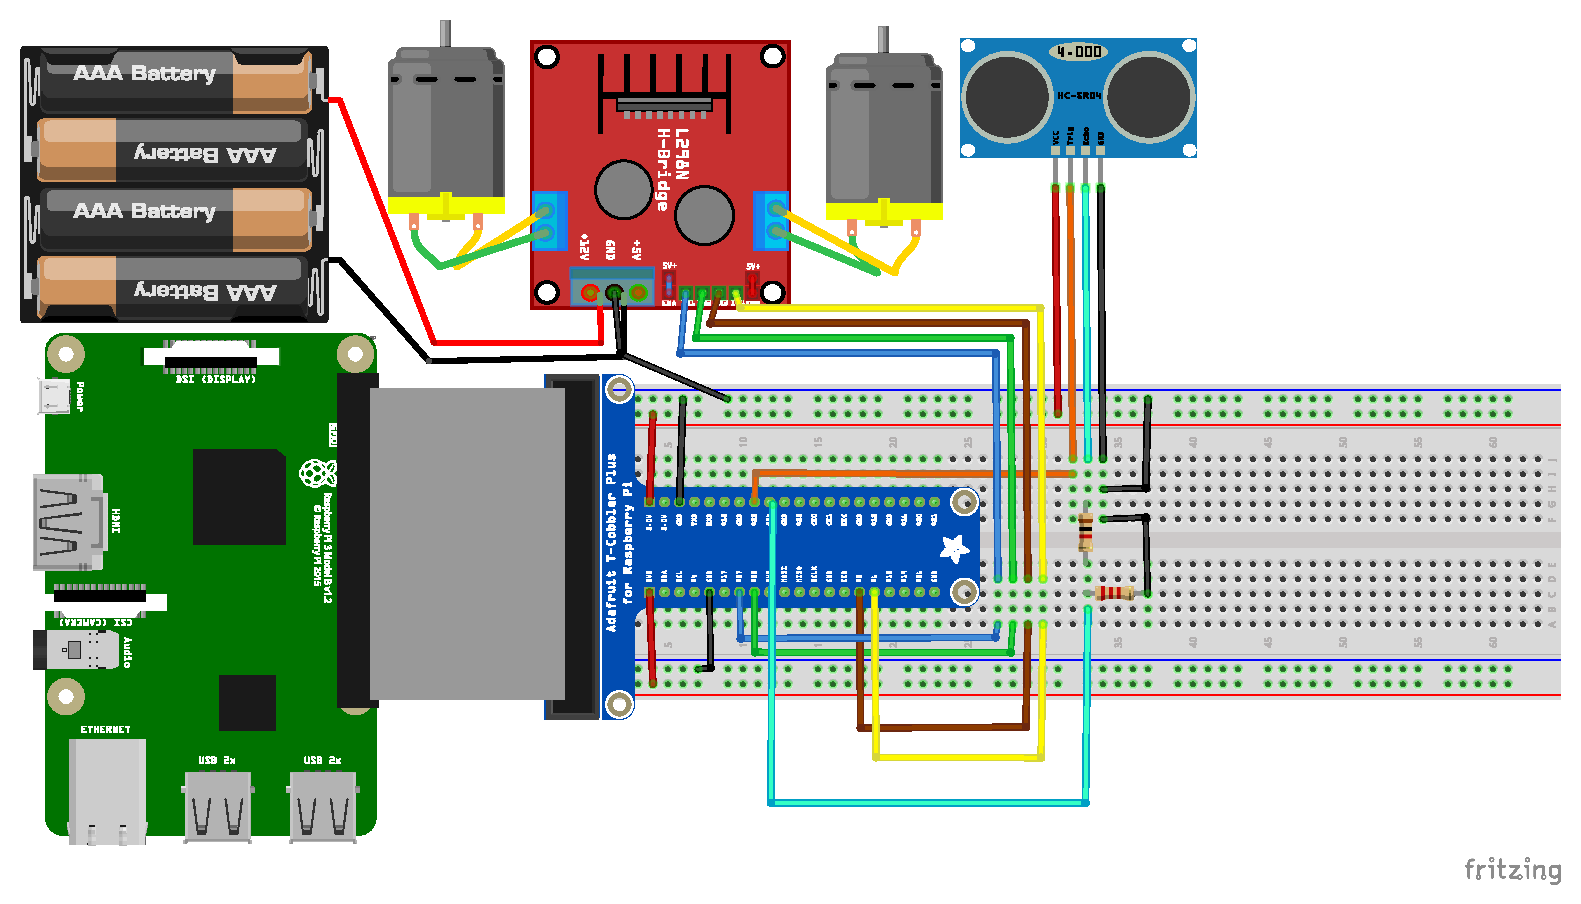
\includegraphics[width=1.2\textwidth]{rover-hwproject}
		\caption[rover-hwproject]{rover-hwproject}
		\label{fig:rover-hwproject}
	\end{figure}
\end{landscape}[]	
\section{Architettura Software}

\section{rpi-rover}
 \lstinputlisting[language={[Sharp]C}]{../rpi-rover/rpi-rover/Program.cs}
\section{rpiservice}
 \lstinputlisting[language={Javascript}]{../rpi-service/rpi-service.js}
\section{fsc-rover}
\lstinputlisting[language={FSharp}]{../fsc-rover/fsc-rover/Program.fs}
